% P05 diagnostic figure reliability_bins|held_evaluation|M06; allowlisted public aggregate points.
% Each point is an aggregate mean or bin over repeated contexts, not an independent sample.
% data_sha256=7f60e425b5fe235c362c21442c3237e1521aad33df8bebdebfd5854e0cfadd4b
\documentclass[tikz,border=5pt]{standalone}
\ifdefined\pdfinfoomitdate\pdfinfoomitdate=1\fi
\ifdefined\pdfsuppressptexinfo\pdfsuppressptexinfo=-1\fi
\ifdefined\pdftrailerid\pdftrailerid{}\fi
\usepackage{pgfplots}
\usepgfplotslibrary{groupplots}
\pgfplotsset{compat=1.18}
\definecolor{p05Blue}{HTML}{0072B2}
\definecolor{p05Orange}{HTML}{E69F00}
\definecolor{p05Green}{HTML}{009E73}
\definecolor{p05Purple}{HTML}{CC79A7}
\definecolor{p05Red}{HTML}{D55E00}
\definecolor{p05Sky}{HTML}{56B4E9}
\begin{document}
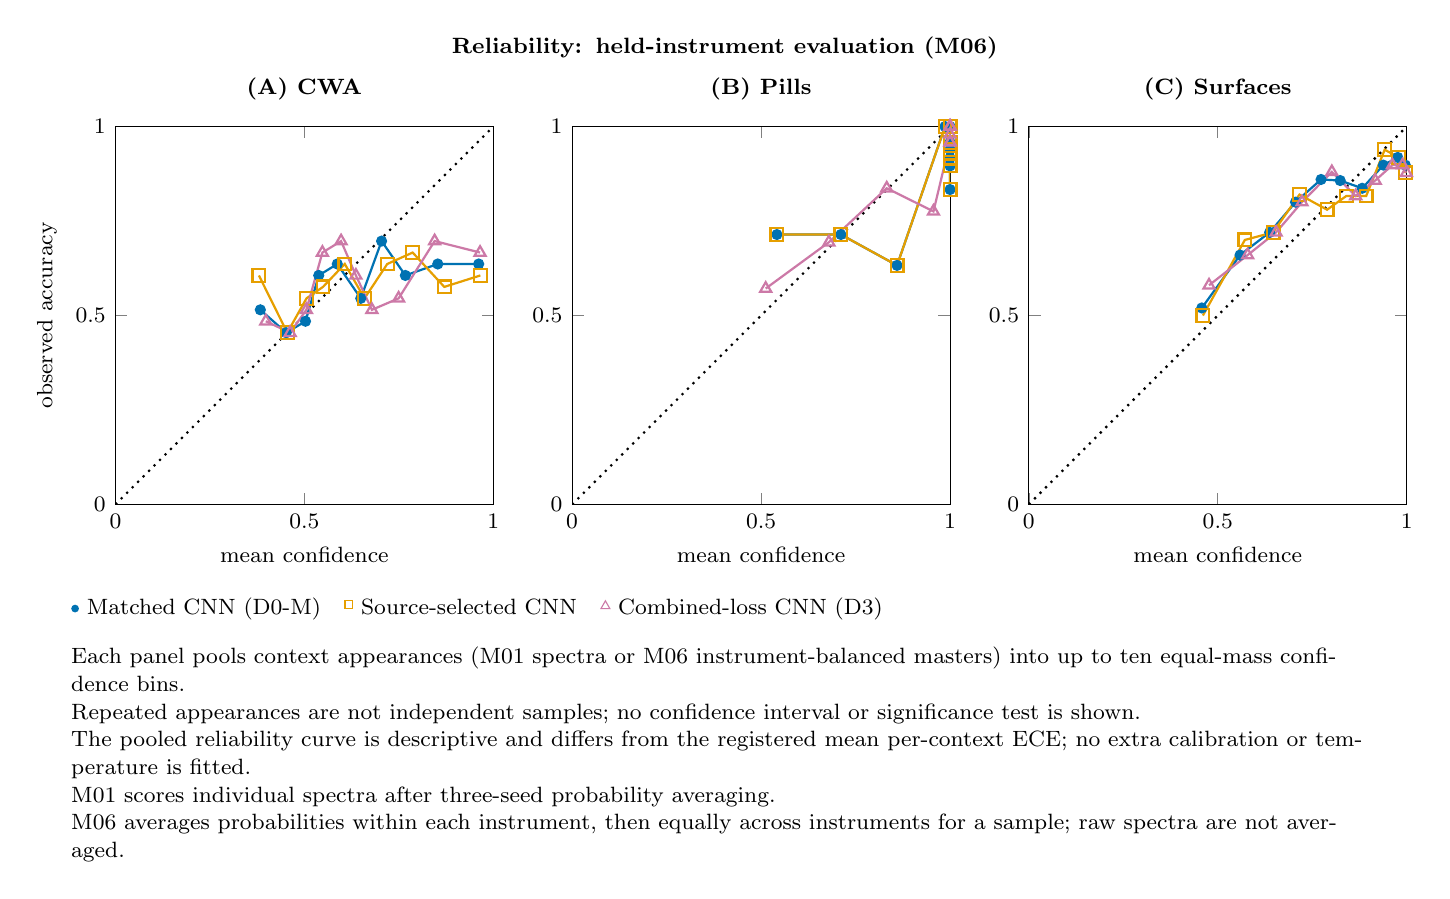
\begin{tikzpicture}
\begin{groupplot}[
  group style={group size=3 by 1, horizontal sep=1.0cm, vertical sep=1.8cm},
  width=4.8cm, height=4.8cm, scale only axis,
  xmin=0, xmax=1, ymin=0, ymax=1,
  xtick={0,0.5,1}, ytick={0,0.5,1},
  tick label style={font=\fontsize{8}{10}\selectfont, color=black},
  label style={font=\fontsize{8}{10}\selectfont, color=black},
  title style={font=\fontsize{8}{10}\selectfont\bfseries, color=black},
]
\nextgroupplot[title={(A) CWA}, xlabel={mean confidence}, ylabel={observed accuracy}]
\addplot[black, dotted, line width=0.8pt] coordinates {(0,0) (1,1)};
\addplot[mark=*, mark size=1.6pt, color=p05Blue, line width=0.8pt, mark options={fill=p05Blue, draw=p05Blue}] coordinates {(0.38343084672906524,0.51515151515151514) (0.45197904792275945,0.45454545454545453) (0.5029936856272661,0.48484848484848486) (0.53795393716916307,0.60606060606060608) (0.587019185503598,0.63636363636363635) (0.6491728107706225,0.54545454545454541) (0.70425959893766044,0.69696969696969702) (0.76716543954860761,0.60606060606060608) (0.85290957504339948,0.63636363636363635) (0.96116953211501777,0.63636363636363635)};
\addplot[mark=square, mark size=2.3pt, color=p05Orange, line width=0.8pt, mark options={fill=none, draw=p05Orange}] coordinates {(0.37960473045159976,0.60606060606060608) (0.45476458589524305,0.45454545454545453) (0.5055732050209254,0.54545454545454541) (0.54921341630421883,0.5757575757575758) (0.6069151026066103,0.63636363636363635) (0.6591169697285526,0.54545454545454541) (0.71922739725705054,0.63636363636363635) (0.78651168293205698,0.66666666666666663) (0.87012811790937561,0.5757575757575758) (0.96562901726945094,0.60606060606060608)};
\addplot[mark=triangle, mark size=2.3pt, color=p05Purple, line width=0.8pt, mark options={fill=none, draw=p05Purple}] coordinates {(0.39792744742552927,0.48484848484848486) (0.46215982329769767,0.45454545454545453) (0.50525972596898017,0.51515151515151514) (0.54766436020449061,0.66666666666666663) (0.59706806974266924,0.69696969696969702) (0.63628696457811063,0.60606060606060608) (0.67861477752918631,0.51515151515151514) (0.74932448839341992,0.54545454545454541) (0.84458976176453759,0.69696969696969702) (0.96482367220952614,0.66666666666666663)};
\nextgroupplot[title={(B) Pills}, xlabel={mean confidence}]
\addplot[black, dotted, line width=0.8pt] coordinates {(0,0) (1,1)};
\addplot[mark=*, mark size=1.6pt, color=p05Blue, line width=0.8pt, mark options={fill=p05Blue, draw=p05Blue}] coordinates {(0.5418884575299634,0.7142857142857143) (0.71110500414194855,0.7142857142857143) (0.85975994284834634,0.63265306122448983) (0.98662048403470248,1) (0.99999970836546859,0.93877551020408168) (0.99999999999600542,0.95833333333333337) (1,0.89583333333333337) (1,1) (1,0.83333333333333337) (1,0.91666666666666663)};
\addplot[mark=square, mark size=2.3pt, color=p05Orange, line width=0.8pt, mark options={fill=none, draw=p05Orange}] coordinates {(0.5418884575299634,0.7142857142857143) (0.71110500414194855,0.7142857142857143) (0.85975994284834634,0.63265306122448983) (0.98662048403470248,1) (0.99999970836546859,0.93877551020408168) (0.99999999999600542,0.95833333333333337) (1,0.89583333333333337) (1,1) (1,0.83333333333333337) (1,0.91666666666666663)};
\addplot[mark=triangle, mark size=2.3pt, color=p05Purple, line width=0.8pt, mark options={fill=none, draw=p05Purple}] coordinates {(0.51221307986844011,0.5714285714285714) (0.67932715329250271,0.69387755102040816) (0.8324609215890888,0.83673469387755106) (0.95609549870817845,0.77551020408163263) (0.99999965057748175,0.95918367346938771) (1,1) (1,0.95833333333333337) (1,1) (1,1) (1,0.97916666666666663)};
\nextgroupplot[title={(C) Surfaces}, xlabel={mean confidence}]
\addplot[black, dotted, line width=0.8pt] coordinates {(0,0) (1,1)};
\addplot[mark=*, mark size=1.6pt, color=p05Blue, line width=0.8pt, mark options={fill=p05Blue, draw=p05Blue}] coordinates {(0.45776311937825137,0.52000000000000002) (0.55896929447005939,0.66000000000000003) (0.63728760632432069,0.71999999999999997) (0.70574663067144228,0.80000000000000004) (0.77332508201736627,0.85999999999999999) (0.82394524643740574,0.8571428571428571) (0.88218535908915396,0.83673469387755106) (0.9381255220841026,0.89795918367346939) (0.9762113570201193,0.91836734693877553) (0.9962093536740908,0.89795918367346939)};
\addplot[mark=square, mark size=2.3pt, color=p05Orange, line width=0.8pt, mark options={fill=none, draw=p05Orange}] coordinates {(0.46065369067085038,0.5) (0.57169963394007195,0.69999999999999996) (0.64634640163471535,0.71999999999999997) (0.71619439021073261,0.81999999999999995) (0.78923950146404209,0.78000000000000003) (0.84019576880000213,0.81632653061224492) (0.89271784289181477,0.81632653061224492) (0.94168923612861744,0.93877551020408168) (0.97824989141415353,0.91836734693877553) (0.99727565138801899,0.87755102040816324)};
\addplot[mark=triangle, mark size=2.3pt, color=p05Purple, line width=0.8pt, mark options={fill=none, draw=p05Purple}] coordinates {(0.47684744347431457,0.57999999999999996) (0.57904761710896679,0.66000000000000003) (0.654275063140493,0.71999999999999997) (0.72281639463796621,0.80000000000000004) (0.80181132494801222,0.88) (0.86490250138018465,0.81632653061224492) (0.91644659077150459,0.8571428571428571) (0.96199216852362923,0.89795918367346939) (0.98891889712418013,0.89795918367346939) (0.9990414895112355,0.87755102040816324)};
\end{groupplot}
\node[anchor=south, font=\fontsize{8}{10}\selectfont\bfseries, color=black, align=center, text width=16.6cm] at (current bounding box.north) {Reliability: held-instrument evaluation (M06)};
\node[anchor=north, font=\fontsize{8}{10}\selectfont, color=black, align=left, text width=16.6cm] (p05legend) at ([yshift=-2mm]current bounding box.south) {\tikz[baseline=-0.6ex]\fill[p05Blue](0,0)circle(1.4pt);\ Matched CNN (D0-M)\quad \tikz[baseline=-0.6ex]\draw[p05Orange](0,0)rectangle(2.8pt,2.8pt);\ Source-selected CNN\quad \tikz[baseline=-0.6ex]\draw[p05Purple](0,0)--(1.6pt,2.8pt)--(3.2pt,0)--cycle;\ Combined-loss CNN (D3)};
\node[anchor=north, font=\fontsize{8}{10}\selectfont, color=black, align=left, text width=16.6cm] at ([yshift=-1mm]p05legend.south) {Each panel pools context appearances (M01 spectra or M06 instrument-balanced masters) into up to ten equal-mass confidence bins.\\Repeated appearances are not independent samples; no confidence interval or significance test is shown.\\The pooled reliability curve is descriptive and differs from the registered mean per-context ECE; no extra calibration or temperature is fitted.\\M01 scores individual spectra after three-seed probability averaging.\\M06 averages probabilities within each instrument, then equally across instruments for a sample; raw spectra are not averaged.};
\end{tikzpicture}
\end{document}
